\documentclass[11pt]{standalone}
\usepackage{tikz}
\usepackage{amssymb}
\begin{document}
% GEOMIRA export: TikZ. One unit is 40.423562bp (53.898083 px on screen).
% Needs \usepackage{tikz} and \usepackage{amssymb}.
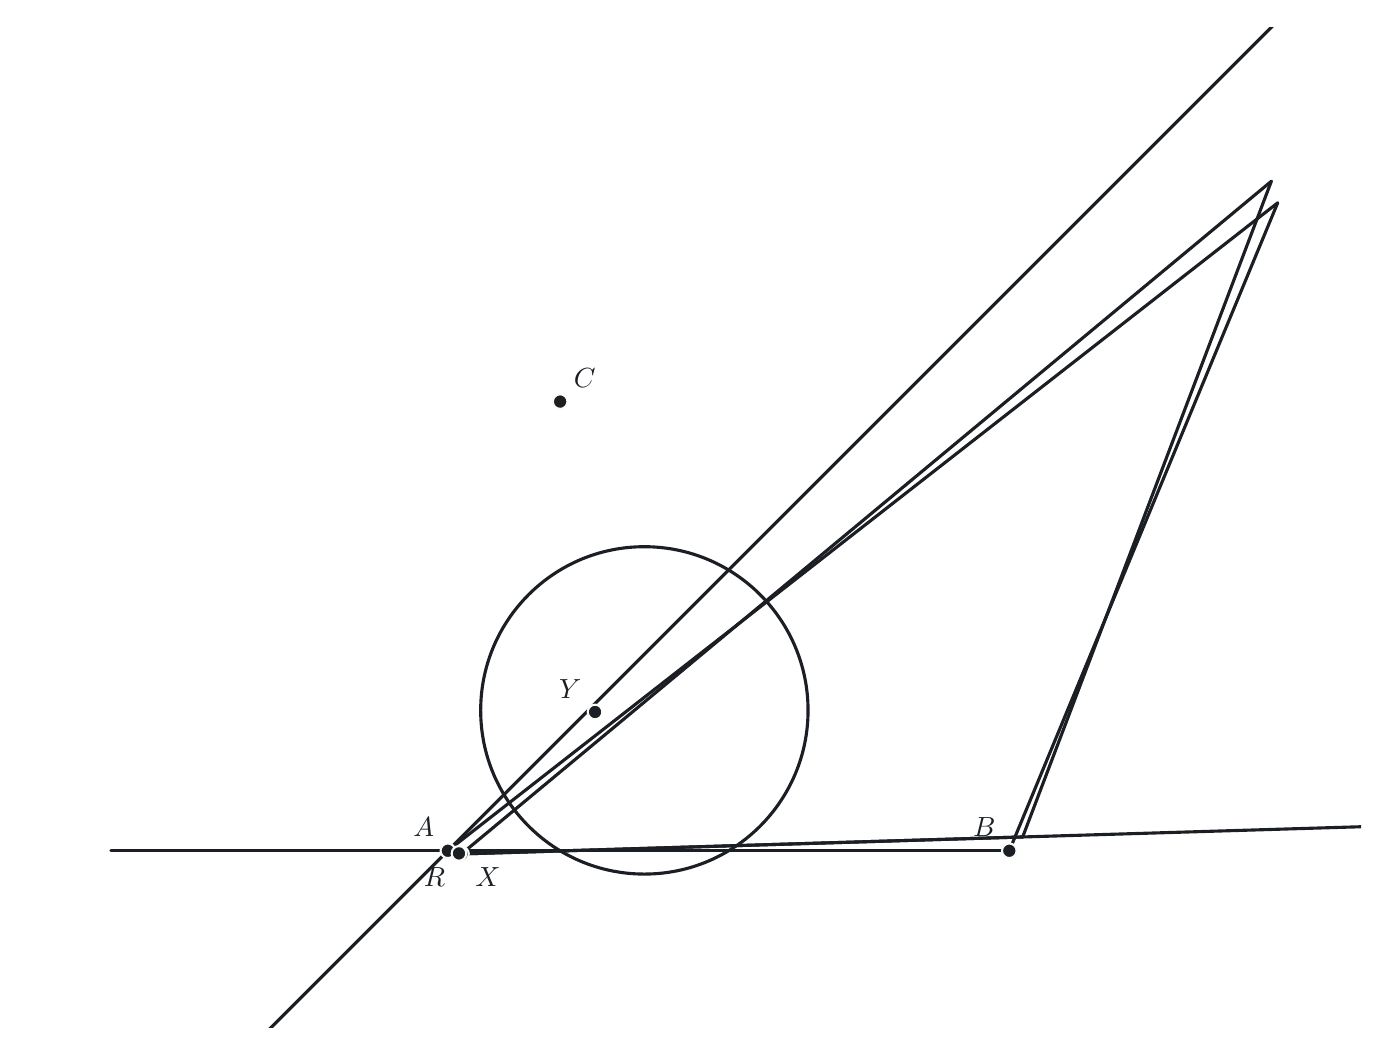
\begin{tikzpicture}[x=40.423562bp, y=40.423562bp, line cap=round, line join=round]
\definecolor{gmc0}{HTML}{1B1F24}
\definecolor{gmc1}{HTML}{FBFBF8}
\clip (-3.7421,-1.5756) rectangle (8.1321,7.3301);
% p
\draw[gmc0, line width=1.125bp] (0,0) -- (5,0);
\draw[gmc0, line width=1.125bp] (5,0) -- (7.39,5.7699);
\draw[gmc0, line width=1.125bp] (7.39,5.7699) -- (0,0);
% q
\draw[gmc0, line width=1.125bp] (0.1214,-0.0284) -- (5.1191,0.1227);
\draw[gmc0, line width=1.125bp] (5.1191,0.1227) -- (7.3336,5.9623);
\draw[gmc0, line width=1.125bp] (7.3336,5.9623) -- (0.1214,-0.0284);
% ν
\draw[gmc0, line width=1.125bp] (3.2077,1.25) arc[start angle=0, end angle=360, radius=1.45774];
% l
\draw[gmc0, line width=1.125bp] (8.5917,8.5917) -- (-2.8372,-2.8372);
% s
\draw[gmc0, line width=1.125bp] (2,0) -- (-3,0);
% r
\draw[gmc0, line width=1.125bp] (0.1214,-0.0284) -- (9.3938,0.252);
% A
\filldraw[fill=gmc0, draw=gmc1, line width=0.75bp] (0,0) circle[radius=2.625bp];
% B
\filldraw[fill=gmc0, draw=gmc1, line width=0.75bp] (5,0) circle[radius=2.625bp];
% C
\filldraw[fill=gmc0, draw=gmc1, line width=0.75bp] (1,4) circle[radius=2.625bp];
% X
\filldraw[fill=gmc0, draw=gmc1, line width=0.75bp] (0.1214,-0.0284) circle[radius=2.625bp];
% R
\filldraw[fill=gmc0, draw=gmc1, line width=0.75bp] (0.099,-0.0235) circle[radius=2.625bp];
% Y
\filldraw[fill=gmc0, draw=gmc1, line width=0.75bp] (1.3107,1.2358) circle[radius=2.625bp];
\node[anchor=south east, inner sep=0pt, text=gmc0] at (-0.1181,0.1181) {$A$}; % label of A
\node[anchor=south east, inner sep=0pt, text=gmc0] at (4.8819,0.1181) {$B$}; % label of B
\node[anchor=south west, inner sep=0pt, text=gmc0] at (1.1181,4.1181) {$C$}; % label of C
\node[anchor=north west, inner sep=0pt, text=gmc0] at (0.2394,-0.1465) {$X$}; % label of X
\node[anchor=north east, inner sep=0pt, text=gmc0] at (-0.019,-0.1415) {$R$}; % label of R
\node[anchor=south east, inner sep=0pt, text=gmc0] at (1.1926,1.3539) {$Y$}; % label of Y
\end{tikzpicture}
\end{document}
